\chapter{Estado del Arte y Marco Teórico}

\section[Fundamentos de la Informática Gráfica]{Fundamentos Históricos de la Informática Gráfica y el Paradigma de la Superficie}
    La evolución de la informática gráfica se ha caracterizado históricamente por intentar alcanzar un mayor realismo visual, exactitud geométrica y rigor físico, lo que ha conllevado el desarrollo de estructuras de datos cada vez más complejas y modelos matemáticos capaces de aprovechar al completo las arquitecturas de hardware de cada época.\\

    En sus inicios, la solución estándar para renderizar los objetos tridimensionales consistió en modelar únicamente la superficie externa, una forma eficiente con un bajo coste computacional pero que presentaba problemas para ciertas simulaciones físicas ya que realmente eran objetos huecos que carecían de densidad.  \\

    Durante las primeras décadas la representación de la estructura 3D de los objetos se llevaba a cabo mediante vértices, que son puntos en el espacio definidos por coordenadas cartesianas (x, y, z) y aristas que los unían. La unión de 3 de estos vértices forma un triángulo, lo que se conoce como cara, que es la unidad fundamental con la que está constituida una malla poligonal (\textit{Boundary Representation} o B-Rep) debido a su eficiencia para la tecnología de la época.\\

    Una vez construida la malla se requiere de un proceso para su visualización conocido como rasterización que consiste en aplicar cálculos espaciales para adaptar los objetos 3D a la perspectiva de la cámara y proyectarlos de forma plana sobre las coordenadas de la pantalla. Una vez que los triángulos están proyectados en el plano 2D el sistema evalúa matemáticamente el área de los triángulos proyectados para identificar qué píxeles concretos quedan cubiertos por ellos. Finalmente, para los píxeles de cada triángulo se le aplica la interacción lumínica siguiendo modelos como el sombreado de Phong o Gouraud,  que calculan la interacción de la luz estimando la reflexión difusa y especular basándose en la normal de la malla. \\
    \begin{figure}[H]
        \centering
        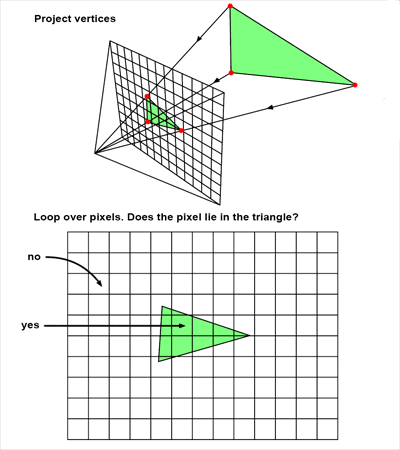
\includegraphics[width=0.6\textwidth]{imagenes/Rasterización.png}
        \caption{Proceso de Rasterización}
        \label{fig:Rasterizacion}
    \end{figure}

    Además de la rasterización otra de las técnica más avanzada era el \textbf{Trazado de Rayos (\textit{Ray Tracing})} que simula el comportamiento de la luz lanzando rayos virtuales desde la cámara a través de cada píxel de la pantalla, buscando la intersección más cercana contra los triángulos del modelo que se encontraba en escena. La principal ventaja de este método frente a la rasterización es la forma en la que hace el cálculo lumínico ya que en lugar de proyectar la geometría en un plano bidimensional para luego aplicar una estimación de la luz, el trazado de rayos realiza una simulación física y espacial directa. Al calcular analíticamente el recorrido exacto de los rayos en el espacio tridimensional, esta técnica logra representar lo fenómenos como reflejos y sombras de una forma más perfecta y realista que no se puede conseguir mediante las aproximaciones que se realizan en la rasterización.\\
    
    Sin embargo, la evolución de sectores como el diseño asistido por ordenador (CAD) y los efectos visuales (VFX) hizo que se fuesen demandando cada vez modelos con formas más orgánicas y realistas que prácticamente no se podían representar con vértices ya que requerían una cantidad enorme que saturaba la limitada capacidad de memoria del hardware. Esta limitación hizo que se comenzaran a utilizar modelos analíticos continuos, consolidando la adopción de los B-Splines Racionales No Uniformes (NURBS).\\

    A diferencia de los triángulos, que representan la geometría con una aproximación con múltiples caras, los NURBS permiten curvar y adaptar la geometría con una alta precisión mediante la manipulación de vértices de control externos y funciones base racionales\\
    \begin{figure}[H]
        \centering
        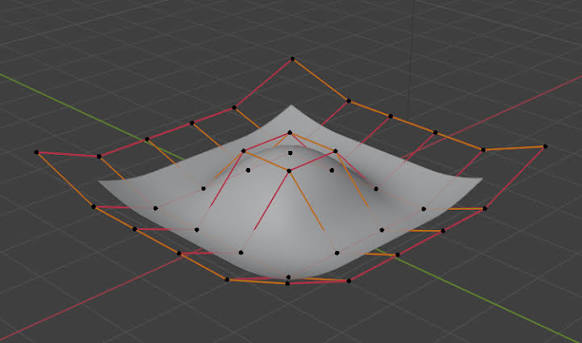
\includegraphics[width=0.6\textwidth]{imagenes/SuperficieNURBS.png}
        \caption[Superficie NURBS]{Superficie NURBS y sus puntos de control}
        \label{fig:burbs}
    \end{figure}
    Pese a esta nueva implementación, tanto las mallas triangulares como las NURBS siguen presentando una gran limitación, solo modelan la superficie exterior, lo que no presenta inconveniente para modelos sólidos y opacos pero sería inviable para intentar representar fenómenos sin fronteras definidas, como el fuego o el humo.\\

    Los primeros intentos de simular dichos fenomenos se realizaron superponiendo capas de polígonos semitransparentes (\textit{alpha-blending}) pero esto fracasó debido a que generaban errores visuales al calcular qué capa estaba delante de otra (\textit{depth-sorting}) y no lograban simular cómo la luz iluminaba el interior del fluido. Para solucionar este problema, pioneros como James Kajiya y Brian Von Herzen demostraron en 1984, con su trabajo fundacional \textit{Ray Tracing Volume Densities}, que era necesario dejar de modelar solo la superficie exterior de los elementos y pasar a un enfoque de modelado volumétrico. Consolidado teóricamente posteriormente por Nelson Max en 1995, el cual transformó conceptualmente el espacio de un simple contenedor pasivo a una matriz tridimensional activa, capaz de almacenar datos continuos de densidad y temperatura en cada punto. \\




\section{Renderizado Volumétrico}
    Para dar una solución visual a las matrices tridimensionales continuas, la informática gráfica tuvo que cambiar drásticamente las técnicas que usaba para el renderizado pasándose a usar métodos de renderizado de volúmenes.\\

    Por una parte tenemos el renderizado de volúmenes indirecto (IVR) que intentan extraer una malla poligonal a partir de los datos espaciales, destacando el algoritmo de \textit{Marching Cubes}.  El funcionamiento de de este algoritmo se basa en analizar el volumen dividiéndolo en cubos lógicos formados por ocho vóxeles vecinos comparando para cada cubo el valor escalar de sus ocho vértices ($v_1, v_2, ..., v_8$) frente a un umbral o iso-valor predefinido ($I$). \\

    Si el valor del vértice comparado es mayor o igual al umbral ($v_i \ge I$), se clasifica como dentro de la superficie (1) mientras que si es menor queda fuera (0), generando así con los 8 vértices una combinación de ceros y unos que se consulta en una tabla precalculada (\textit{look-up table}) en la que se indica exactamente qué configuración de triángulos debe dibujarse dentro de ese cubo.\\
    \begin{figure}[H]
        \centering
        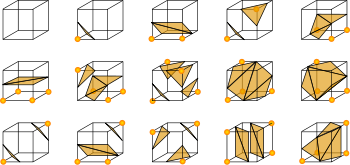
\includegraphics[width=0.6\textwidth]{imagenes/MarchingCubesCases.png}
        \caption[Formación de MarchingCubes]{Posibles casos de MarchingCubes}
        \label{fig:MarchingCubesCases}
    \end{figure}

    Sin embargo, esta técnica presenta dos limitaciones críticas. 
    \begin{itemize}
        \item Su complejidad algoritmica hace que necesite realizar una enorme cantidad de cálculos computacionales para generar mallas de alta resolución.
        \item   Su función principal es construir una frontera artificial que envuelve los datos, lo que le impide visualizar las estructuras internas y las continuas variaciones de densidad.
    \end{itemize}

    Por este motivo, para el renderizado de fenómenos como el humo o el agua se optó por el Renderizado Volumétrico Directo (DVR) que al contrario que el IVD sí permite visualizar el interior de los volúmenes y no necesita generar ninguna geometría intermedia ahorrandole esa carga computacional. Para lograr esto, se desarrolló el Trazado de Rayos Volumétrico (\textit{Volumetric Ray Tracing}), una técnica donde los rayos generados desde la cámara ya no buscan colisionar contra una superficie externa, sino que atraviesan directamente todo el volumen de datos, calculando la absorción y dispersión de la luz en su interior.\\

    La implementación algorítmica y optimizada de esta técnica en tiempo real se conoce como \textit{Raymarching}. Es un algoritmo que en lugar de procesar todo el volumen de golpe, lanza un rayo desde la cámara hacia el volumen el cual cada cierta distancia va tomando muestras de los valores del voxel en el que se encuentre, como densidad o temperatura, para ir sumándolos y calcular el color final del píxel hasta que el rayo abandona el volumen o se vuelve completamente opaco.\\

    Para calcular el color final resultante para un píxel se resuelve mediante la siguiente ecuación discreta:\\

    $$
    C_{total} = \sum_{i=0}^{N} C_i \alpha_i \prod_{j=0}^{i-1} (1 - \alpha_j)
    $$

    Donde las variables son:
    \begin{itemize}
        \item \textbf{$C_{total}$}: Es el color final y opacidad resultante que se mostrará en el píxel de la pantalla.
        \item \textbf{$C_i \alpha_i$}: Representa la contribución de color radiante ($C_i$) ponderada por su propia opacidad o densidad local ($\alpha_i$) en el paso exacto $i$ en el que se encuentra el rayo.
        \item \textbf{$\prod_{j=0}^{i-1} (1 - \alpha_j)$}: Es el porcentaje de luz que logró sobrevivir y llegar hasta el paso $i$. Lo hace multiplicando la transparencia inversa ($1 - \alpha$) de todos los pasos anteriores ($j$) que el rayo ya ha atravesado.
    \end{itemize}

    Hasta este punto, técnicas como el DVR y el \textit{Raymarching} funcionan sin problema para la visualización de una matriz tridimensional estática pero para simular fluidos naturales y fenómenos como el humo o el fuego es necesario dotar a ese volumen de movilidad y dinámicas físicas en tiempo real.\\

    Para lograr esta movilidad en tiempo real, se tuvo que trasladar la carga computacional a la tarjeta gráfica debido al alto número de cálculos y actualizaciones que se necesitan, mapeando la cuadrícula espacial del renderizado sobre texturas tridimensionales alojadas en la memoria de vídeo (VRAM).\\
    %\textit{GPU Gems 3} (NVIDIA, 2007)
    \begin{figure}[H]
        \centering
        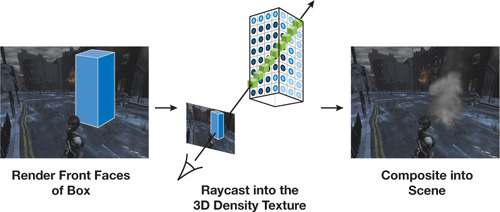
\includegraphics[width=0.9\textwidth]{imagenes/RenderDVR.png}
        \caption[Trazado de Rayos]{Descripción conceptual del trazado de rayos}
        \label{fig:RenderDVR}
    \end{figure}
    Aprovechando la arquitectura de la GPU, en lugar de calcular trayectorias de partículas individuales, se utiliza programas  con una alta capacidad de paralelizar cálculos, como los \textit{Compute} o \textit{Fragment Shaders}, y así evaluar simultáneamente millones de celdas estáticas. Dado que la GPU no permite leer y escribir sobre el mismo bloque de memoria de forma segura al mismo tiempo se mantener dos texturas 3D idénticas donde en cada iteración el \textit{shader} lee los datos de una y escribe el resultado en la segunda, cambiando los roles en el siguiente ciclo. Esta técnica es conocida como \textbf{\textit{Ping-Ponging}}.\\

    Una vez que la infraestructura de memoria está lista para la actualización dinámica y paralela, se necesitaba definir un marco matemático que gobernase su evolución temporal. Para ello se recurre a la investigación operativa a través de los \textbf{Autómatas Celulares}, los cuales se adaptan perfectamente al funcionamiento del \textit{Raymarching} y permiten evaluar cada celda espacial de forma iterativa mediante reglas de transición basadas en su situación actual y en las condiciones de sus vóxeles adyacentes. \\

    Finalmente al juntar estas dos técnicas se consigue transformar un contenedor volumétrico estático en un ecosistema reactivo idóneo para la creación de simuladores en tiempo real como los de incendios forestales. \\


\section[Modelos Físicos de Propagación]{Modelos Físicos de Propagación de Incendios Forestales}
    El estudio de la propagación y el avance de los incendios forestales se ha fundamentado históricamente en la necesidad de predecir el comportamiento del fuego para la gestión de emergencias. \\

    Las primeras aproximaciones analíticas, que siguen siendo el estándar en la actualidad, se basaron en modelos matemáticos empíricos destacando el modelo cuasi-estacionario de Rothermel (1972), el cual calcula la tasa de propagación frontal ($R$) del fuego basándose en la carga física del combustible, la topografía y la meteorología:\\

    $$R = \frac{I_R \xi}{\rho_b \epsilon Q_{ig}}$$

    Esta formulación divide la velocidad de propagación entre las fuerzas de empuje térmico y los sumideros de energía, que representan la resistencia de las plantas al tener que absorber calor para evaporar su humedad antes de prenderse. Sus variables principales son:
    \begin{itemize}
        \item \textbf{$I_R$ (Intensidad de reacción):} Energía bruta liberada por unidad de área activa.
        \item \textbf{$\xi$ (Flujo de calor propagado):} Fracción de energía convectiva/radiante proyectada hacia la vegetación frontal intacta.
        \item \textbf{$\rho_b$ (Densidad aparente):} Masa de la biomasa por volumen.
        \item \textbf{$\epsilon$ (Calentamiento efectivo):} Eficiencia térmica de absorción.
        \item \textbf{$Q_{ig}$ (Calor de pre-ignición):} Energía necesaria para evaporar la humedad y alcanzar la pirólisis.
    \end{itemize}


    Posteriormente, en la década de 1980 y principios de 1990, se estandarizó como gran alternativa internacional el Sistema Canadiense de Predicción del Comportamiento del Fuego (FBP) que, a diferencia del balance energético de Rothermel, es estrictamente empírico. Se apoya en bases de datos masivas obtenidas de quemas controladas y de la observación de incendios forestales reales en bosques boreales, usando estos datos para relacionar directamente la velocidad de propagación empírica con el tipo de combustible topográfico y el Índice Meteorológico de Peligro de Incendio (FWI, \textit{Fire Weather Index}) a través de ecuaciones de regresión, ofreciendo resultados muy precisos en ecosistemas concretos.\\

    La ecuación principal para determinar la tasa de propagación base según el modelo FBP se define como:
    $$ROS = a \cdot (1 - e^{-b \cdot ISI})^c$$
    En esta formulación, a diferencia del modelo de Rothermel  los componentes son puramente estadísticos y meteorológicos:
    \begin{itemize}
        \item \textbf{$a, b, c$ (Constantes de regresión):} Son coeficientes empíricos precalculados para cada uno de los 16 modelos de combustible estándar definidos en Canadá (como coníferas, frondosas o pastos).
        \item \textbf{$ISI$ (\textit{Initial Spread Index}):} Es un valor numérico del sistema FWI que combina la velocidad del viento con el contenido de humedad de los combustibles finos y que representa el potencial de propagación inmediato del fuego sin tener en cuenta la acumulación de combustible pesado.
    \end{itemize}

    Finalmente, esta propagación base se ajusta multiplicándola por un factor de efecto de acumulación, que introduce la influencia del combustible forestal de mayor grosor. Al basarse en coeficientes de regresión es computacionalmente mucho más ligero que Rothermel, por lo cual sistemas, como el simulador nacional canadiense \textit{Prometheus}, pueden calcular grandes expansiones de forma muy ágil, aunque perdiendo la capacidad de usarse en ecosistemas para los que no existan grandes cantidades de datos estadísticos previos.\\

    Tanto las ecuaciones de Rothermel como las del FBP calculan la propagación en un punto específico de forma unidimensional por lo que la simulación espacial determinista de los años 90 adoptó técnicas de propagación vectorial basadas en el \textbf{Principio de Huygens}. Este principio, originario de la física ondulatoria, establece que cada punto de un frente de onda actúa como un nuevo emisor de ondas secundarias, siendo la suma de todos los bordes de estas ondas secundarias la que forman la siguiente onda grande. \\

    Al adaptar este concepto matemático a los incendios forestales, el frente de onda es la línea de fuego donde se asume que cada punto activo se comporta como un foco de ignición independiente que genera su propia área de propagación. La envolvente exterior de todas estas áreas conforma el perímetro actualizado del incendio, permitiendo simular con gran precisión expansiones asimétricas, flancos que avanzan a distinta velocidad y cambios abruptos en la dirección del viento sin que el frente del fuego se rompa matemáticamente.\\

    A partir de la fusión de estos modelos de propagación han surgido distintos simuladores que dominan la gestión de emergencias a nivel mundial. Por un lado, sistemas como \textit{FARSITE} y \textit{BehavePlus}, desarrollados por el Servicio Forestal de EE. UU., utilizan el modelo matemático físico de Rothermel combinado con la propagación elíptica de Huygens. Por otro lado, \textit{Prometheus}, el simulador nacional de Canadá, emplea el mismo motor de propagación vectorial de Huygens pero alimentado matemáticamente por las ecuaciones empíricas de su propio sistema nacional (FBP). \\

    En el panorama nacional español resalta la labor del Laboratorio de Defensa contra Incendios Forestales de la Universidad de Córdoba (LABIF-UCO), el cual bajo el liderazgo del Dr. Francisco Rodríguez y Silva, ha desarrollado sistemas como UCO40, que cataloga 40 modelos de combustible superficial para afinar el comportamiento térmico de Rothermel en formaciones endémicas andaluzas.\\

    De forma paralela, otros enfoques más modernos han optado por la Dinámica de Fluidos Computacional (CFD) para resolver las complejas ecuaciones espaciales de Navier-Stokes aplicadas a la combustión y la convección térmica. Sin embargo, tanto los modelos de expansión vectorial como los sistemas CFD tienen una gran limitación práctica: su altísimo coste computacional hace imposible una simulación a gran escala en tiempo real, ofreciendo además salidas puramente analíticas (mapas isócronos de contornos 2D) sin inmersión visual para los operativos.\\

    \subsection{Autómatas Celulares}

        Para superar estos cuellos de botella computacionales que provocan los modelos continuos y vectoriales, y permitir así simulaciones dinámicas sobre grandes extensiones de terreno, la investigación evolucionó hacia modelos basados en cuadrículas discretas,  mediante el uso de Autómatas Celulares (CA). \\

        Un autómata celular es un modelo matemático compuesto por una matriz regular de celdas donde cada una posee un estado perteneciente a un conjunto finito de posibilidades (en el contexto forestal, típicamente: intacto, en ignición, ardiendo o calcinado). El funcionamiento se basa en la evolución iterativa de todo el sistema, para cada iteración temporal, el nuevo estado de una celda se calcula aplicando un conjunto definido de reglas de transición que evalúan tanto sus condiciones internas como el estado de las celdas adyacentes que conforman su vecindad (normalmente las ocho celdas que la rodean en el caso de un plano bidimensional,  lo que se conoce como vecindad de Moore). 

        Esta arquitectura se puede trasladar a fenómenos complejos como la propagación de un gran frente de llamas a partir de interacciones locales al depender únicamente de su entorno más inmediato. Esto logra que la actualización del estado de cada celda sea totalmente independiente del resto del mapa, lo que convierte a los autómatas celulares en estructuras ideales para ser paralelizadas masivamente en sistemas de cómputo modernos.\\

        El enfoque contemporáneo más aceptado es el modelo estocástico propuesto por Alexandridis et al. (2008) cuya precisión quedó demostrada al simular a posteriori incendios devastadores como el de Spetses (1990) y Rodas (2008), prediciendo áreas quemadas con un margen de error mínimo y sin reajustes artificiales.\\

        En este modelo, la probabilidad de ignición ($P_{ign}$) temporal de una celda sana vecina a una celda en llamas se define como:
        $$P_{ign} = P_0 \cdot (1 + p_w) \cdot (1 + p_s) \cdot p_h$$

        Esta ecuación desglosa la termodinámica de Rothermel en multiplicadores independientes que pueden procesarse en paralelo para millones de celdas de forma instantánea:
        \begin{itemize}
            \item \textbf{$P_0$ (Probabilidad Base):} Representa la inflamabilidad inherente al tipo de combustible forestal.
            \item \textbf{$p_w$ (Factor de Viento):} Se calcula exponencialmente, penalizando o bonificando la propagación según si el viento sopla a favor o en contra de la celda vecina:
            $$p_w = \exp(c_1 \cdot V \cdot (\cos(\theta) - 1))$$
            Donde $V$ es la velocidad del viento, $\theta$ es el ángulo entre la dirección del viento y la línea de propagación, y $c_1$ es la constante empírica de ponderación del viento.
            \item \textbf{$p_s$ (Factor de Pendiente):} Refleja cómo la convección térmica precalienta el combustible de forma más eficiente cuesta arriba:
            $$p_s = \exp(a \cdot \tan(\theta_s))$$
            Donde $\theta_s$ es el ángulo de inclinación del terreno local y $a$ es la constante empírica de pendiente.
            \item \textbf{$p_h$ (Factor de Humedad):} Se encarga de frenar el avance del fuego, ya que el agua contenida en la vegetación debe evaporarse antes de alcanzar la pirólisis. Se modela como un decaimiento exponencial:
            $$p_h = \exp(- c_2 \cdot H)$$
            Donde $H$ es el índice de humedad relativa (de $0$ a $1$) y $c_2$ es la constante de resistencia térmica a la humedad.\\

        \end{itemize}
        
        \begin{table}[H]
            \centering
            \footnotesize
            \renewcommand{\arraystretch}{1.5}
            \makebox[\textwidth][c]{
                \begin{tabular}{|l|c|p{6.5cm}|}
                    \hline
                    \textbf{Parámetro CA de Alexandridis} & \textbf{Valor Típico} & \textbf{Definición} \\ \hline
                    Constante de Viento ($c_1$) & $0.045$ & Ponderación del flujo convectivo. \\ \hline
                    Constante de Humedad ($c_2$) & $0.131$ & Resistencia térmica a la humedad. \\ \hline
                    Constante de Pendiente ($a$) & $0.078$ & Constante empírica de la pendiente. \\ \hline
                    Probabilidad Base ($P_0$) & $0.580$ & Probabilidad base bajo condiciones de referencia mediterráneas. \\ \hline
                \end{tabular}
            }
            \caption[Valores empíricos para el Autómata Celular]{Valores empíricos de calibración para el Autómata Celular basados en el incendio de Spetses.}
            \label{tab:parametros_alexandridis}
        \end{table}

    \subsection{Método de Monte Carlo}
        A pesar de los avances en los modelos empíricos y los Autómatas Celulares, la predicción de incendios forestales se enfrenta a otro problema fundamental. Variables importantes como la velocidad y dirección del viento o el grado de humedad del combustible rara vez se conocen con precisión y en muchas de las ocasiones sufren cambios repentinos que pueden conllevar a un comportamiento del fuego totalmente distinto al calculado inicialmente.\\

        Para resolver esta vulnerabilidad se pasó de usar un enfoque determinista, donde se produce un único resultado que ignora la variabilidad del entorno, a predicciones probabilísticas utilizando el Método de Montecarlo. 
        Este método consiste en ejecutar la simulación de propagación del fuego un número elevado de veces ($N$ iteraciones), introduciendo en cada una de ellas pequeñas variaciones aleatorias en los parámetros de entrada dentro de un rango de varianza estadística controlada.\\

        Al agrupar los resultados, se obtiene un  mapa de riesgo donde la probabilidad de que una celda espacial sea alcanzada por el fuego se define como la razón entre el número de simulaciones en las que dicha celda ardió y el total de iteraciones:
        $$P_{quemado}(x,y,z) = \frac{1}{N} \sum_{i=1}^{N} S_i(x,y,z)$$

        Donde $N$ es el número total de simulaciones del conjunto y $S_i(x,y,z)$ indica el estado final de la celda en la iteración $i$ (siendo $1$ si fue quemada y $0$ si permaneció intacta).\\ 

        Hoy en día, la potencia de las GPU permite ejecutar estas predicciones en tiempo real lo que permite que dos grandes beneficios:\\
        \begin{itemize}
            \item \textbf{Evaluación de riesgos a largo plazo:} Ejecutando miles de igniciones aleatorias sobre grandes escalas de paisaje para identificar áreas críticas o cuellos de botella topográficos, generando lo que se conoce como Mapas de Probabilidad de Quema (\textit{Burn Probability Maps}).

        \item \textbf{Predicción operativa en tiempo real :} Durante una emergencia activa puede simular múltiples escenarios futuros de un mismo incendio para reasignar recursos de una manera eficiente minimizando pérdidas.

        \end{itemize}

        No obstante, aunque estos sistemas mejoraron la velocidad de cálculo, la visualización seguía estando limitada en gran medida a entornos bidimensionales o representaciones topográficas esquemáticas. \\
        \begin{figure}[H]
            \centering
            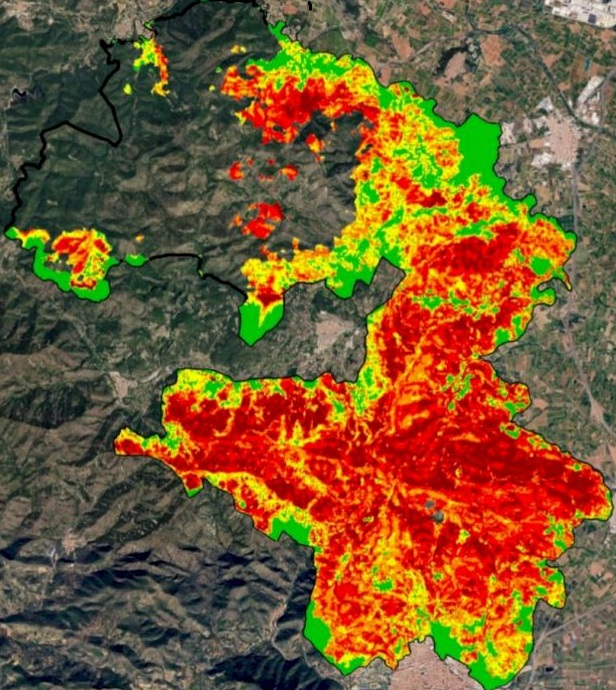
\includegraphics[width=0.6\textwidth]{imagenes/MapaCalorIncendio.png}
            \caption{Ejemplo de mapa de calor 2D de un incendio}
            \label{fig:MapaCalor}
        \end{figure}
    A pesar de los grandes avances tanto en el renderizado 3D como en el cálculo de las probabilidades de incendios  todavía nos encontramos con una gran desconexión entre ellos. Por un lado, los simuladores forestales científicos, nutridos con rigor termodinámico, carecen de representaciones volumétricas inmersivas que dificultan la comprensión del volumen y la orografía real, mientras que por el otro ,la industria gráfica y los motores de videojuegos disponen de una avanzada tecnología de renderizado volumétrico en tiempo real pero que  pero generan sus fluidos alimentando las ecuaciones ópticas mediante algoritmos de ruido procedimental.\\

    Este proyecto propone fusionar ambos paradigmas, desarrollando un simulador interactivo en el motor Godot 4 que delegue la lógica matemática de propagación basada en Autómatas Celulares a la GPU mediante el uso de \textit{Compute Shaders}. Además de usar Modelos Digitales de Elevación reales (\textit{Heightmaps}) como entorno físico y \textit{Raymarching} como técnica de renderización volumétrica, consiguiendo así una herramienta con un rigor matemático de la prevención de incendios y fidelidad visual.\\
